\documentclass[dutch]{report}
\usepackage[utf8]{inputenc}
\usepackage{babel}

\usepackage{titling}
\usepackage{graphicx}
\usepackage[utf8]{inputenc}

\usepackage{internship-docs-styling/style/a4-document-setup}
\usepackage{internship-docs-styling/style/internship-styling}

\author{Mies van der Lippe \& Roel Huizing}
\title{IKPMD I StayConnected App}

\renewcommand{\versiondate}{17-03-2020}
\renewcommand{\versionnumber}{0.5.1}
\renewcommand{\versionname}{Ontwikkelversie}

\usepackage{enumitem}

\begin{document}
	
	\begin{titlepage}
	
	\stylizedtitle
	\stylizedauthor
	\titlepageversion
	
	\vfill
	
	\begin{tabular}{rl}
		Student 1 & Mies van der Lippe \hspace{1cm}S1096607\\
		Student 2 & Roel Huizing \hfill S1092755\\
		Vak		  & IKPMD \\
	\end{tabular}
	
	\vspace{10mm}
	
	\hfill
	\includegraphics[height=1.5cm]{internship-docs-styling/img/hsl.png}	
	
\end{titlepage}
	\tableofcontents

	\newpage
	
	\section{Inleiding}
	
	\subsection{Leerdoelen}
	De student kan:
	\begin{enumerate}
		\item Een omgeving gebruiken voor ontwikkeling voor Android apparaten.
		\item Interne en externe opslag gebruiken op een Android apparaat.
		\item Een lijst met element maken gevuld met data van een externe locatie.
		\item Een inzichtelijke visualisatie van data maken in een Android app.
		\item Een API of firebase opzetten en gebruiken vanuit een app.
		\item Een grafisch interface ontwerpen en realiseren voor een Android apparaat.
		\item Een versioning systeem beschrijven, opzetten en gebruiken. 
		\item Een app realiseren voor een Androidapparaat met een gegeven casus of op basis van een eigen voorstel.
	\end{enumerate}

	\subsection{Eindeisen}
	\begin{enumerate}[label=\Alph*:]
		\item Student begrijpt versioning systematiek en gebruikt deze voor de opdracht.
		\item Student werkt met de belangrijkste tools binnen een ontwikkelomgeving.
		\item Student maaktverschillendeinterface elementen voor een app.
		\item Student slaat data van de appop.
		\item Student beschrijft zijn app in een verslag
		\item Student richt een API of Firebase invoor gebruik met de app.
		\item Correct aanleveren van een werkende app en een goed verslag
	\end{enumerate}

	\newpage
	
	\section{Productverslag}
	%% Een productverslag met screenshots van alle schermen. 
	%% Hier staat beschreven hoe de app werkt en welke (on)mogelijkheden de app heeft. Verder bevat het 
	%% productverslag o.a.op welke versie van de Android SDK is ontwikkeld,in hoeverre het MAVEN build 
	%% script is aangepast voor de applicatiemet een kleine uitleg, screenshots van de network statistics, 
	%% CPU-loaden memory usage opgenomen uit de DDMS.
	
	\section{Wat is StayConnected eigenlijk?}
	Tekst
	
	\newpage
	
	\section{Design}
	%% Een beschrijving van de gemaakte interface elementen, zoals buttons, invoervelden, toast msg 
	%% en/of snackbars. Er wordt een versie van een lijstgemaakt(bijvoorbeeld de ListView) Er wordt 
	%% gebruik gemaakt van parameter passing. Er wordt een manier van data visualisatiegemaakt om 
	%% gegevens inzichtelijk te maken.Tevens beschijf je kort hoe je material design hebt toegepast 
	%% in je app.
	
	
	\subsection{Het menu}
	Voor deze app is gebruik gemaakt van de app met menu template. In het menu worden de verschillende 
	mogelijkheden van de app getoond. Voor de account optie is een apart icoon gemaakt, voor de andere
	twee is gekozen voor iets dat in de buurt komt van een passend icoon en dat al in het template zat. 
	
	Zoals te zien is wordt de tekst bij het account aangepast als de gebruiker inlogt. 
	
	\begin{minipage}{0.50\textwidth}
		\begin{center}
			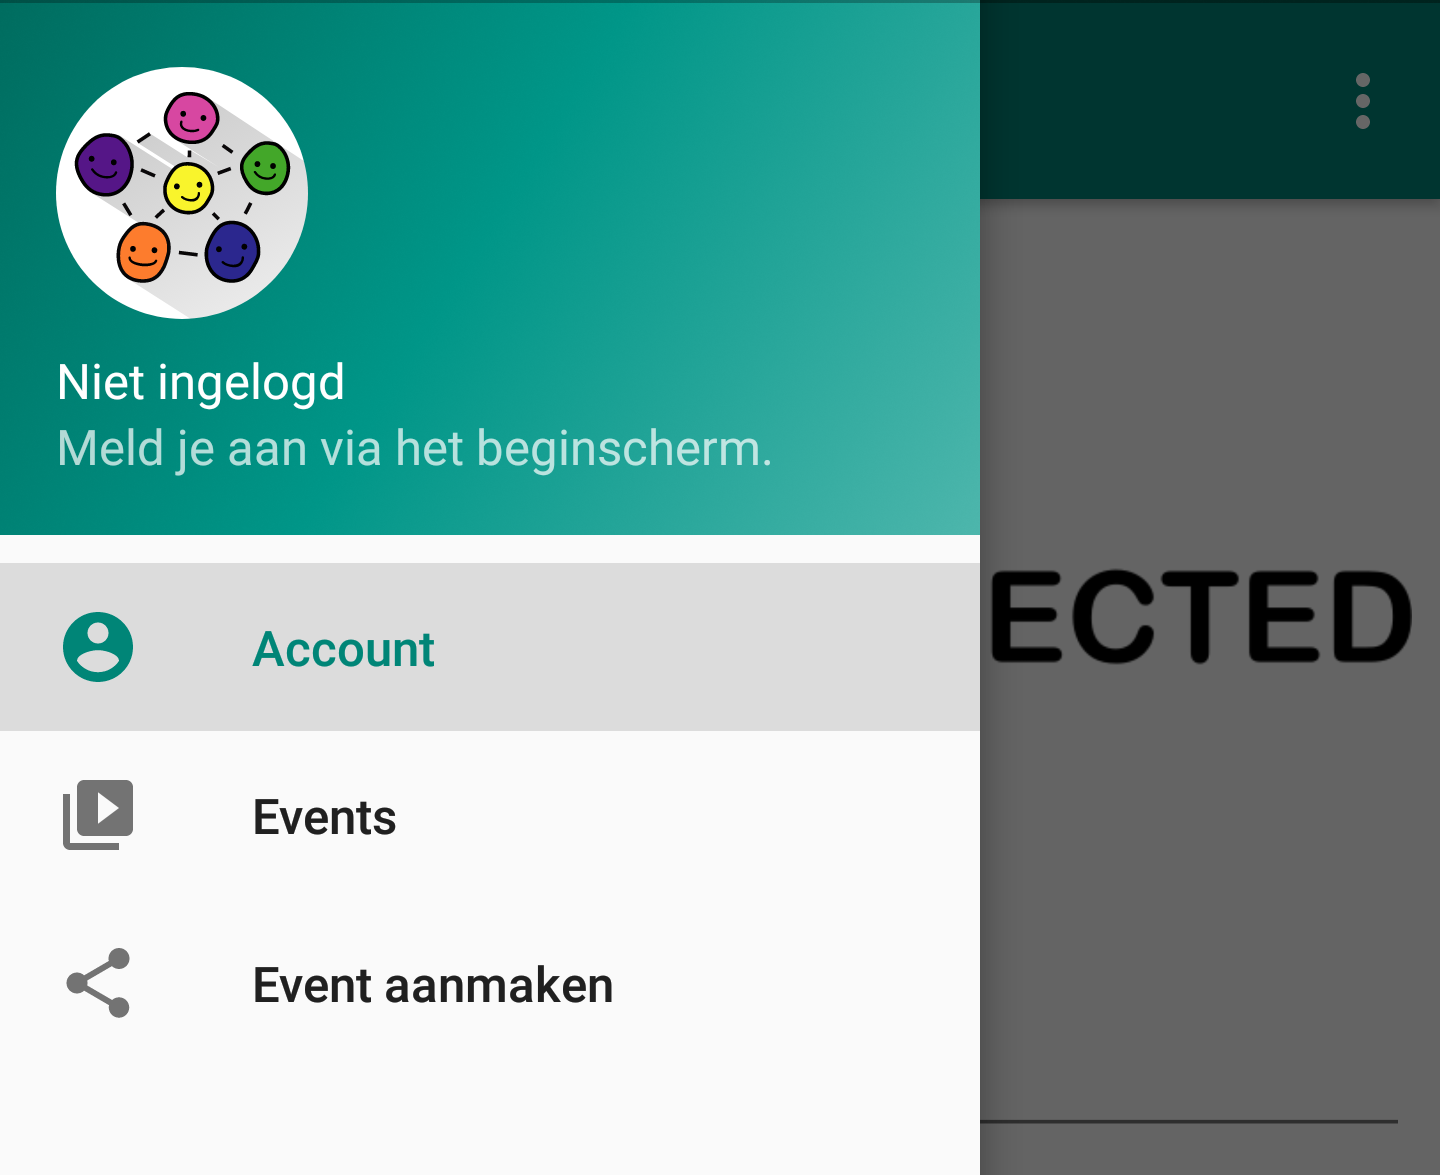
\includegraphics[width=5cm]{images/nietingelogd.png}		
		\end{center}
	\end{minipage}
	\hfill
	\begin{minipage}{0.50\textwidth}
		\begin{center}
			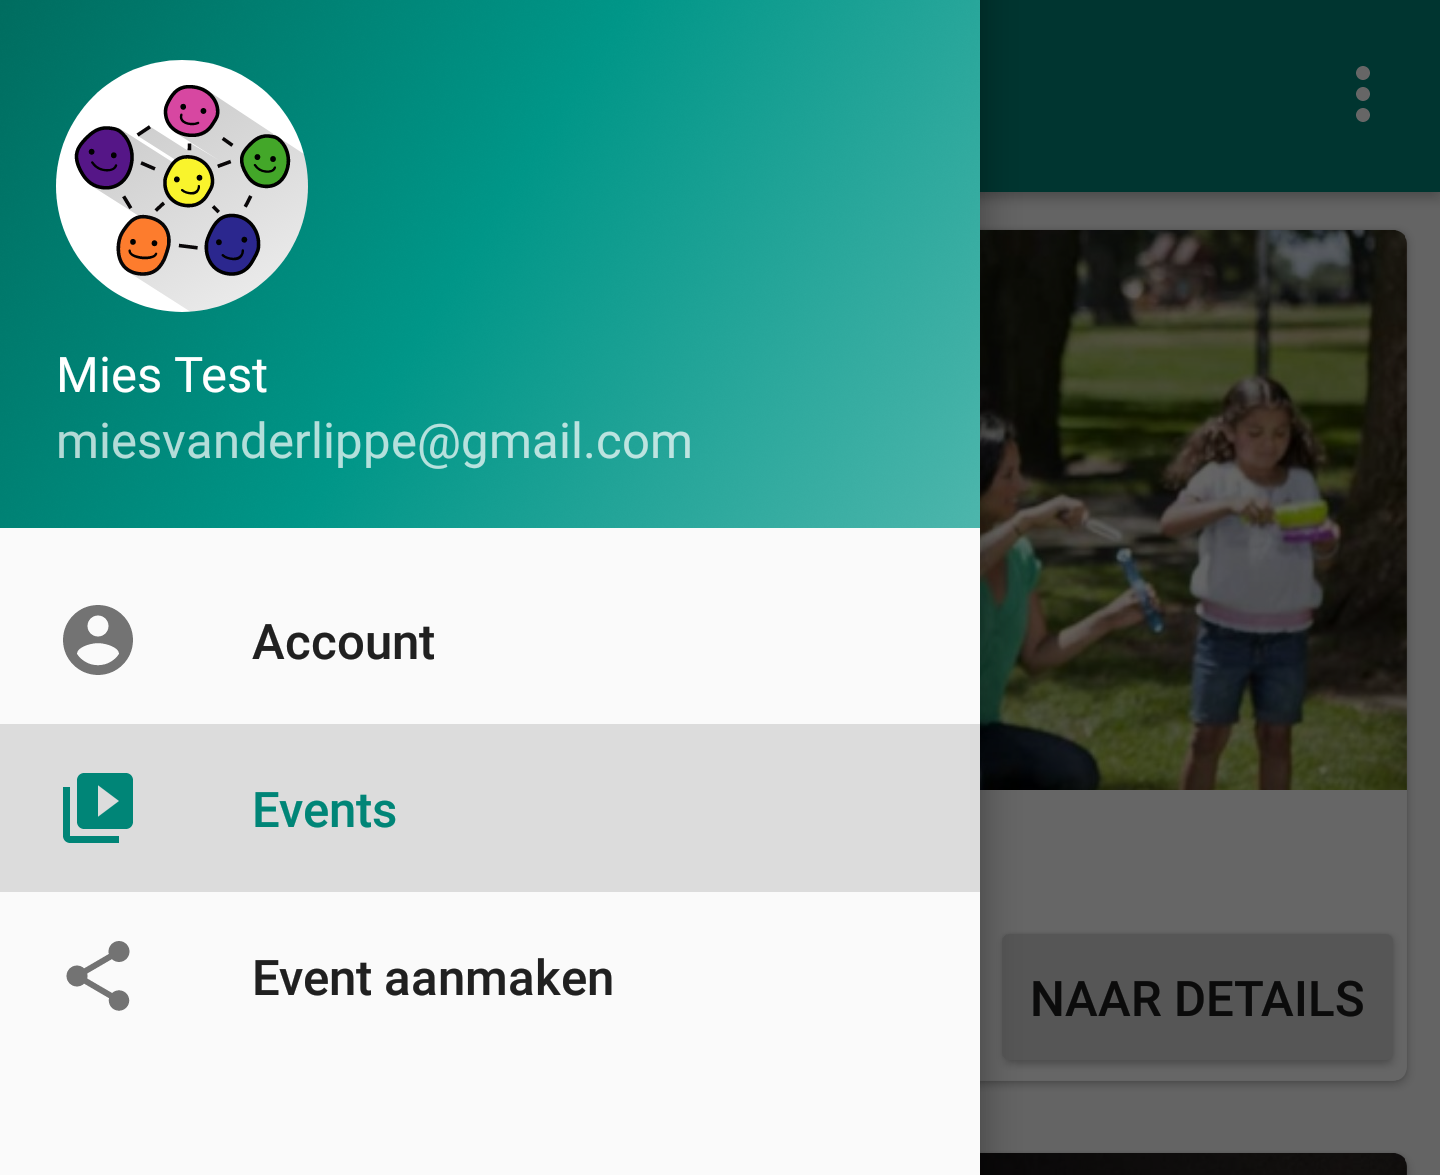
\includegraphics[width=5cm]{images/ingelogd.png}
		\end{center}
	\end{minipage}
	
	
	\subsection{De evenementen lijst}
	\begin{minipage}{0.60\textwidth}
	Een belangrijk design element in deze app is de lijst met kaartjes waarin de evenementen weergegeven
	worden. De combinatie van een afbeelding, tekst en knop geven veel ruimte voor het toepassen van de 
	richtlijnen en grafische elementen. 
	
	Zoals te zien is heeft de kaart een kleine 'hoogte' om zo een ruimtelijk effect te geven. De hoeken 
	zijn enigszins afgerond zonder dat het kitscherig wordt. De afbeelding vult het kaartje tot aan de 
	rand, wat rustiger is dan een randje eromheen laten. 
	
	Technisch is het een RecyclerView met daarin Cardviews, een RelativeLayout, een ImageView, wat 
	teksten en een knop.
	
	\end{minipage}
	\hfill
	\begin{minipage}{0.35\textwidth}
	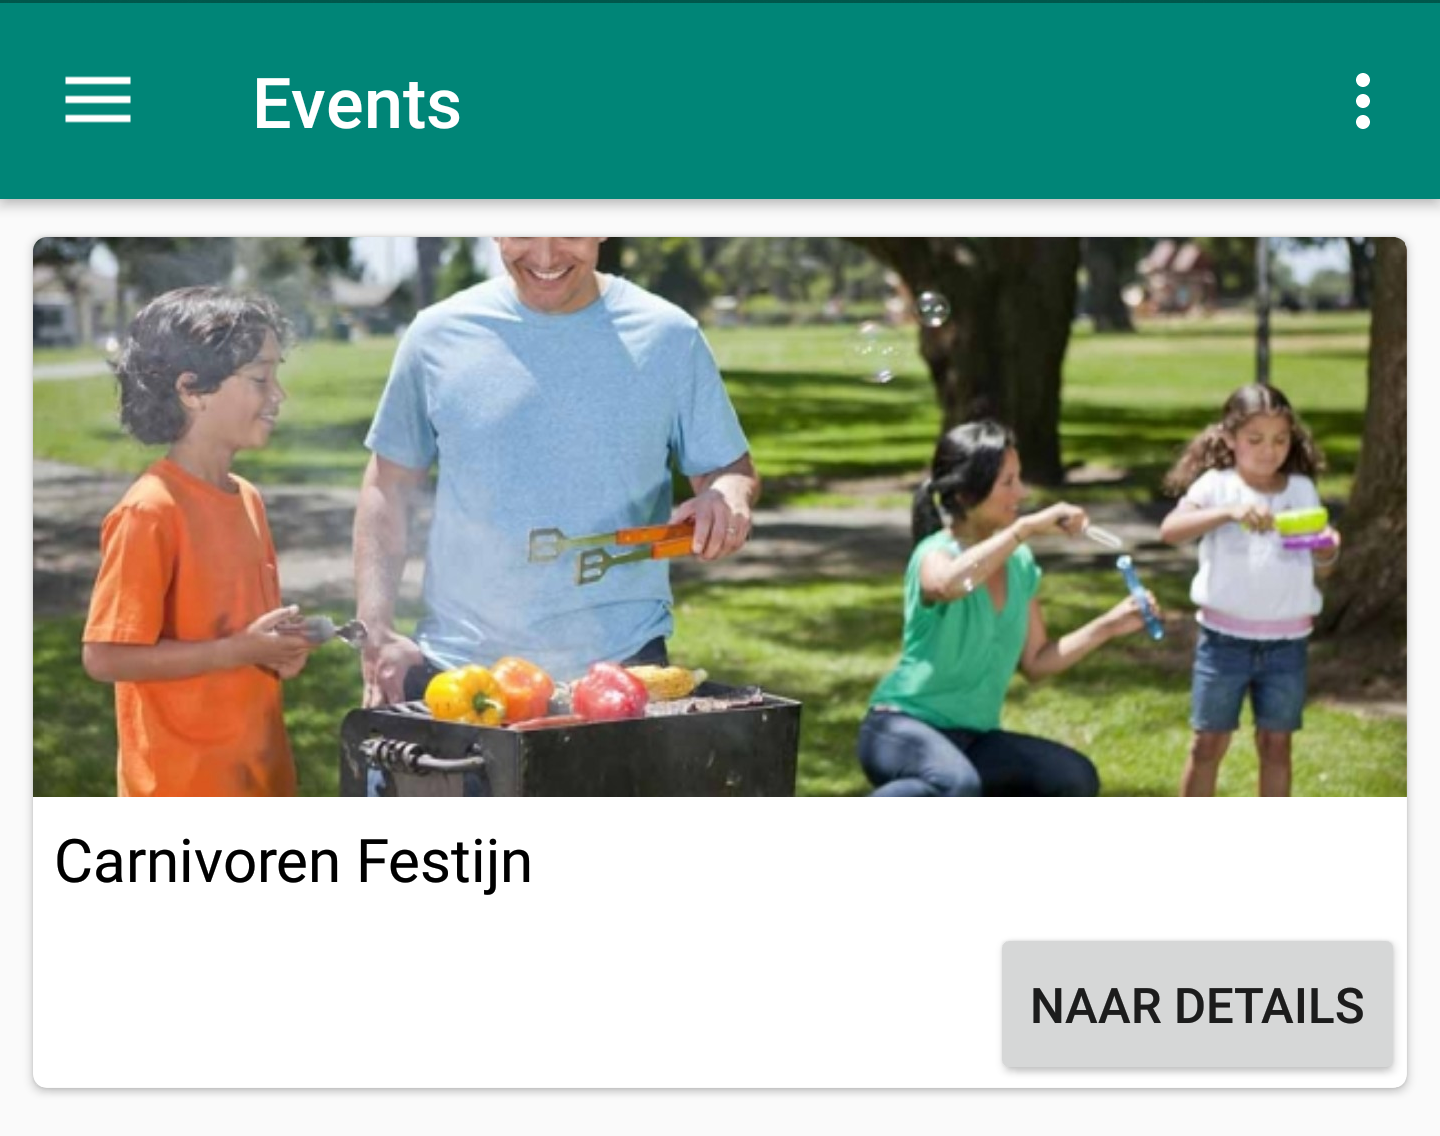
\includegraphics[width=\linewidth]{images/cardlist.png}
	\end{minipage}
	
	\subsection{Het account}
	Een gebruiker kan in- en uitloggen. Hier wordt gebruik gemaakt van de hints in de tekstinvoer. Voor 
	de rest is het een vrij eenvoudige layout. 
	
	\begin{minipage}{0.50\textwidth}
		\begin{center}
			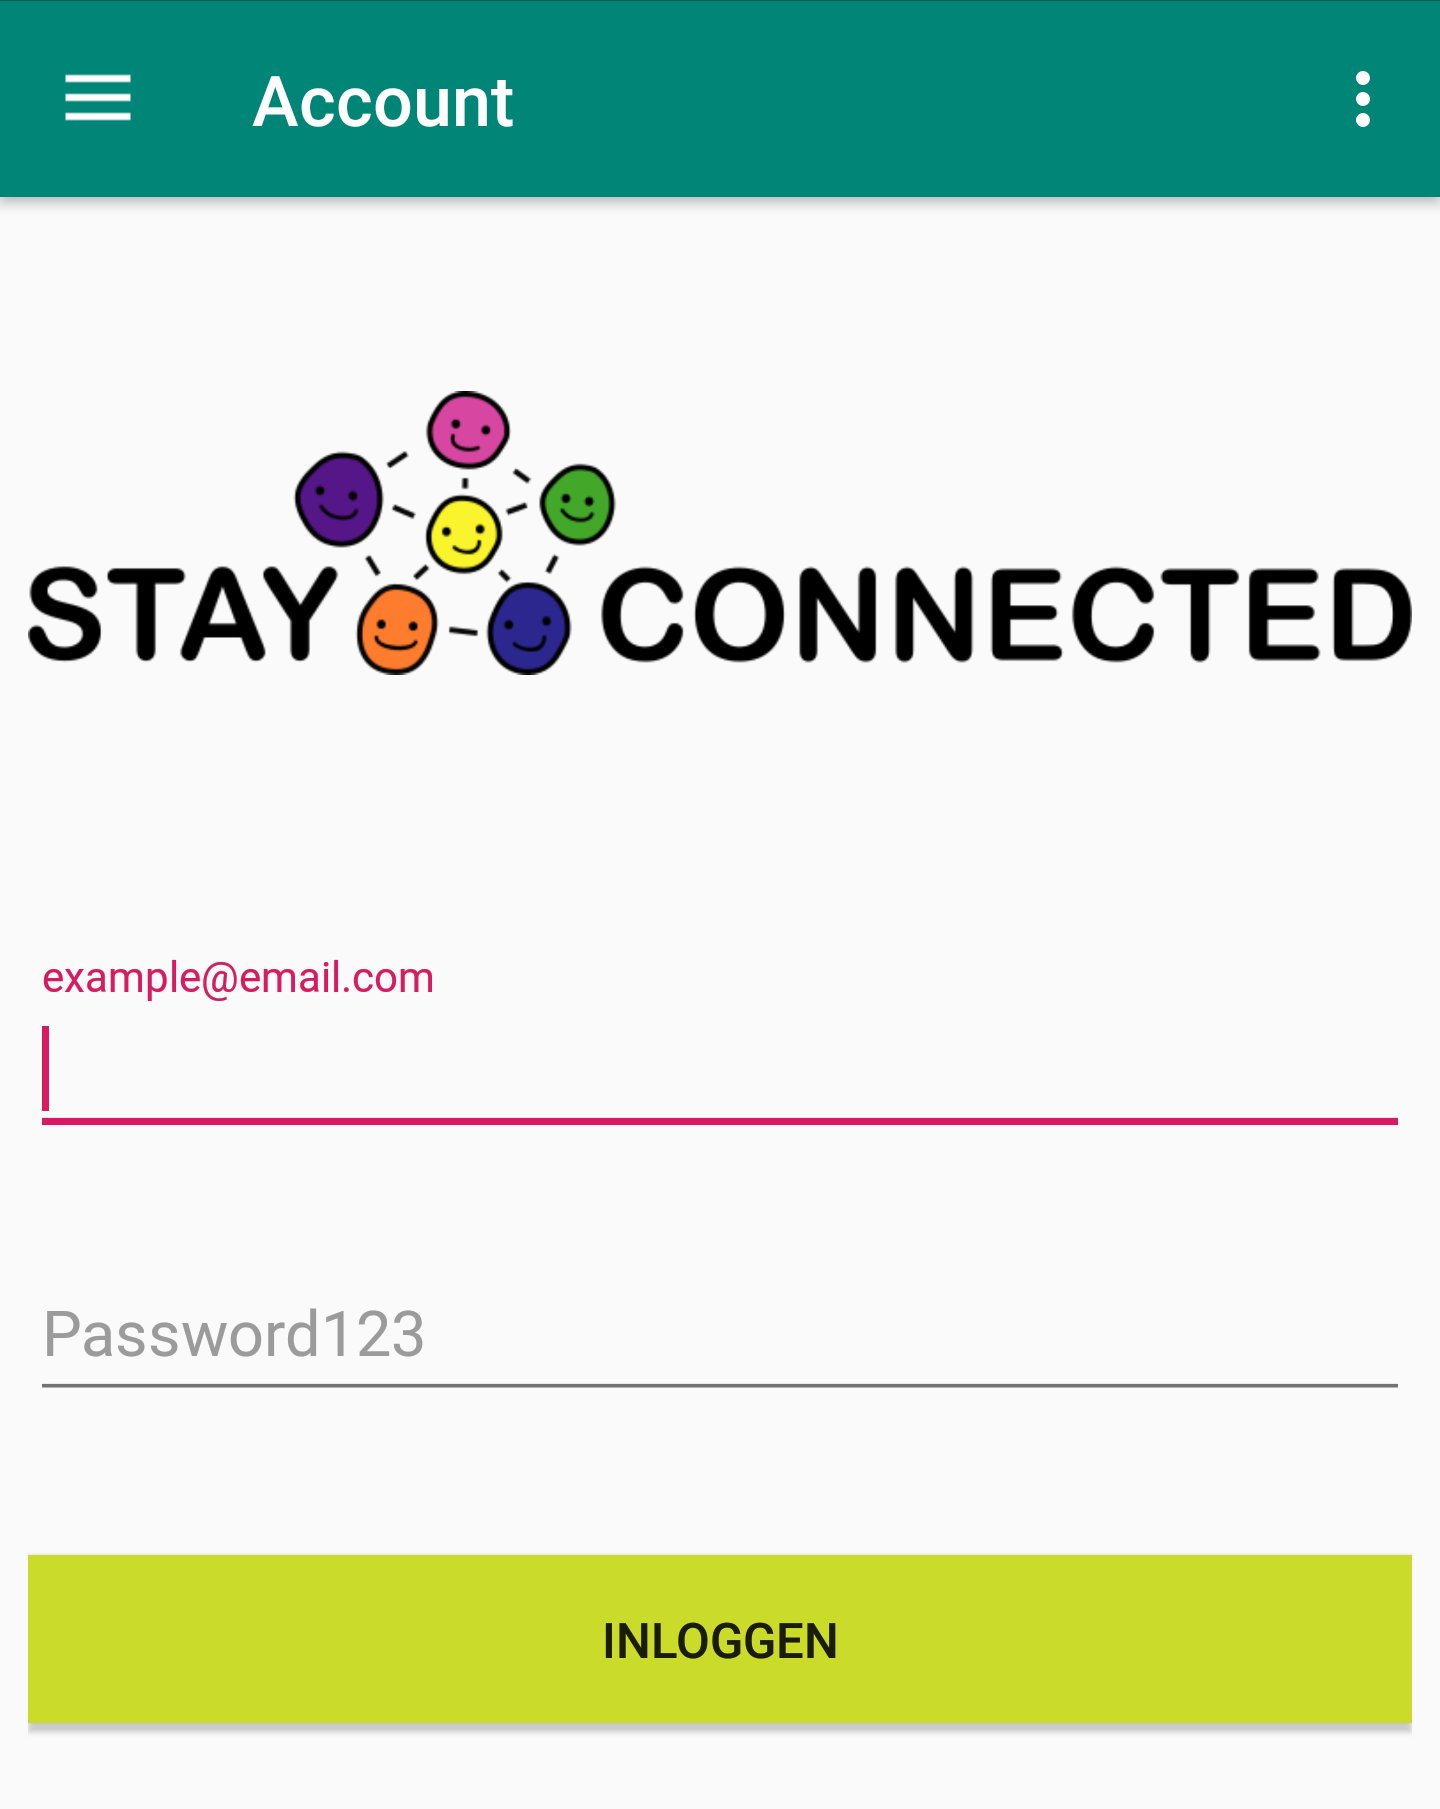
\includegraphics[width=5cm]{images/inloggen.png}		
		\end{center}
	\end{minipage}
	\hfill
	\begin{minipage}{0.50\textwidth}
		\begin{center}
			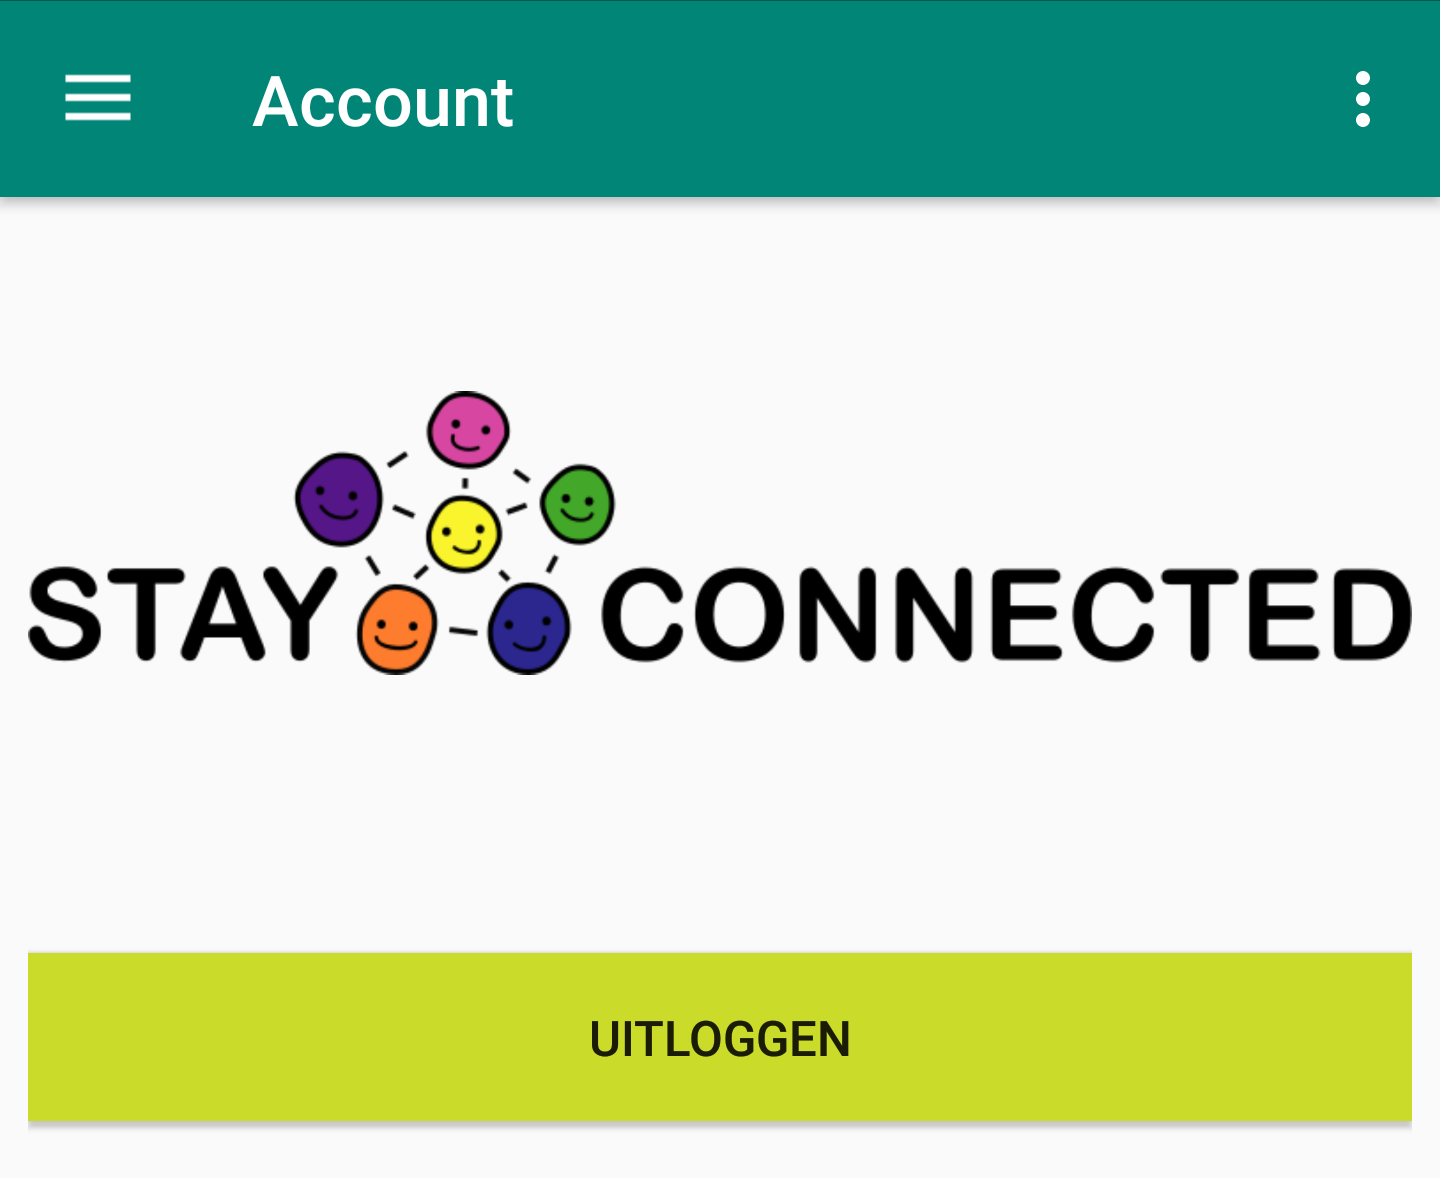
\includegraphics[width=5cm]{images/uitloggen.png}
		\end{center}
	\end{minipage}
	
	
	\subsection{De detailpagina}
	\begin{minipage}{0.60\textwidth}
	Een gebrek aan design is ook design toch? Voor de detailpagina is gekozen voor een robuste, eenvoudige
	weergave. Voor de deelname knop wordt na het laden de status van inschrijving opgehaald. Op basis daarvan
	wordt het een deelnemen- of verlaten- knop. De knop wordt dus ook verborgen voor niet ingelogde gebruikers
	of wanneer er geen verbinding is. Ook de balk bovenin is weggelaten omdat het idee is dat deze informatie
	over de app heen ligt. Als de inhoud te lang wordt, kan de gebruiker scrollen. 
	
	Deze weergave bevat vooral informatie uit het EventData object. Deze wordt geserializeerd en meegegeven 
	via de intent informatie bundel. De informatie over deelname wordt naderhand opgehaald aan de hand van 
	centraal geregelde informatie over de ingelogde gebruiker, en een repository voor evenementen. 
	
	\end{minipage}
	\hfill
	\begin{minipage}{0.35\textwidth}
		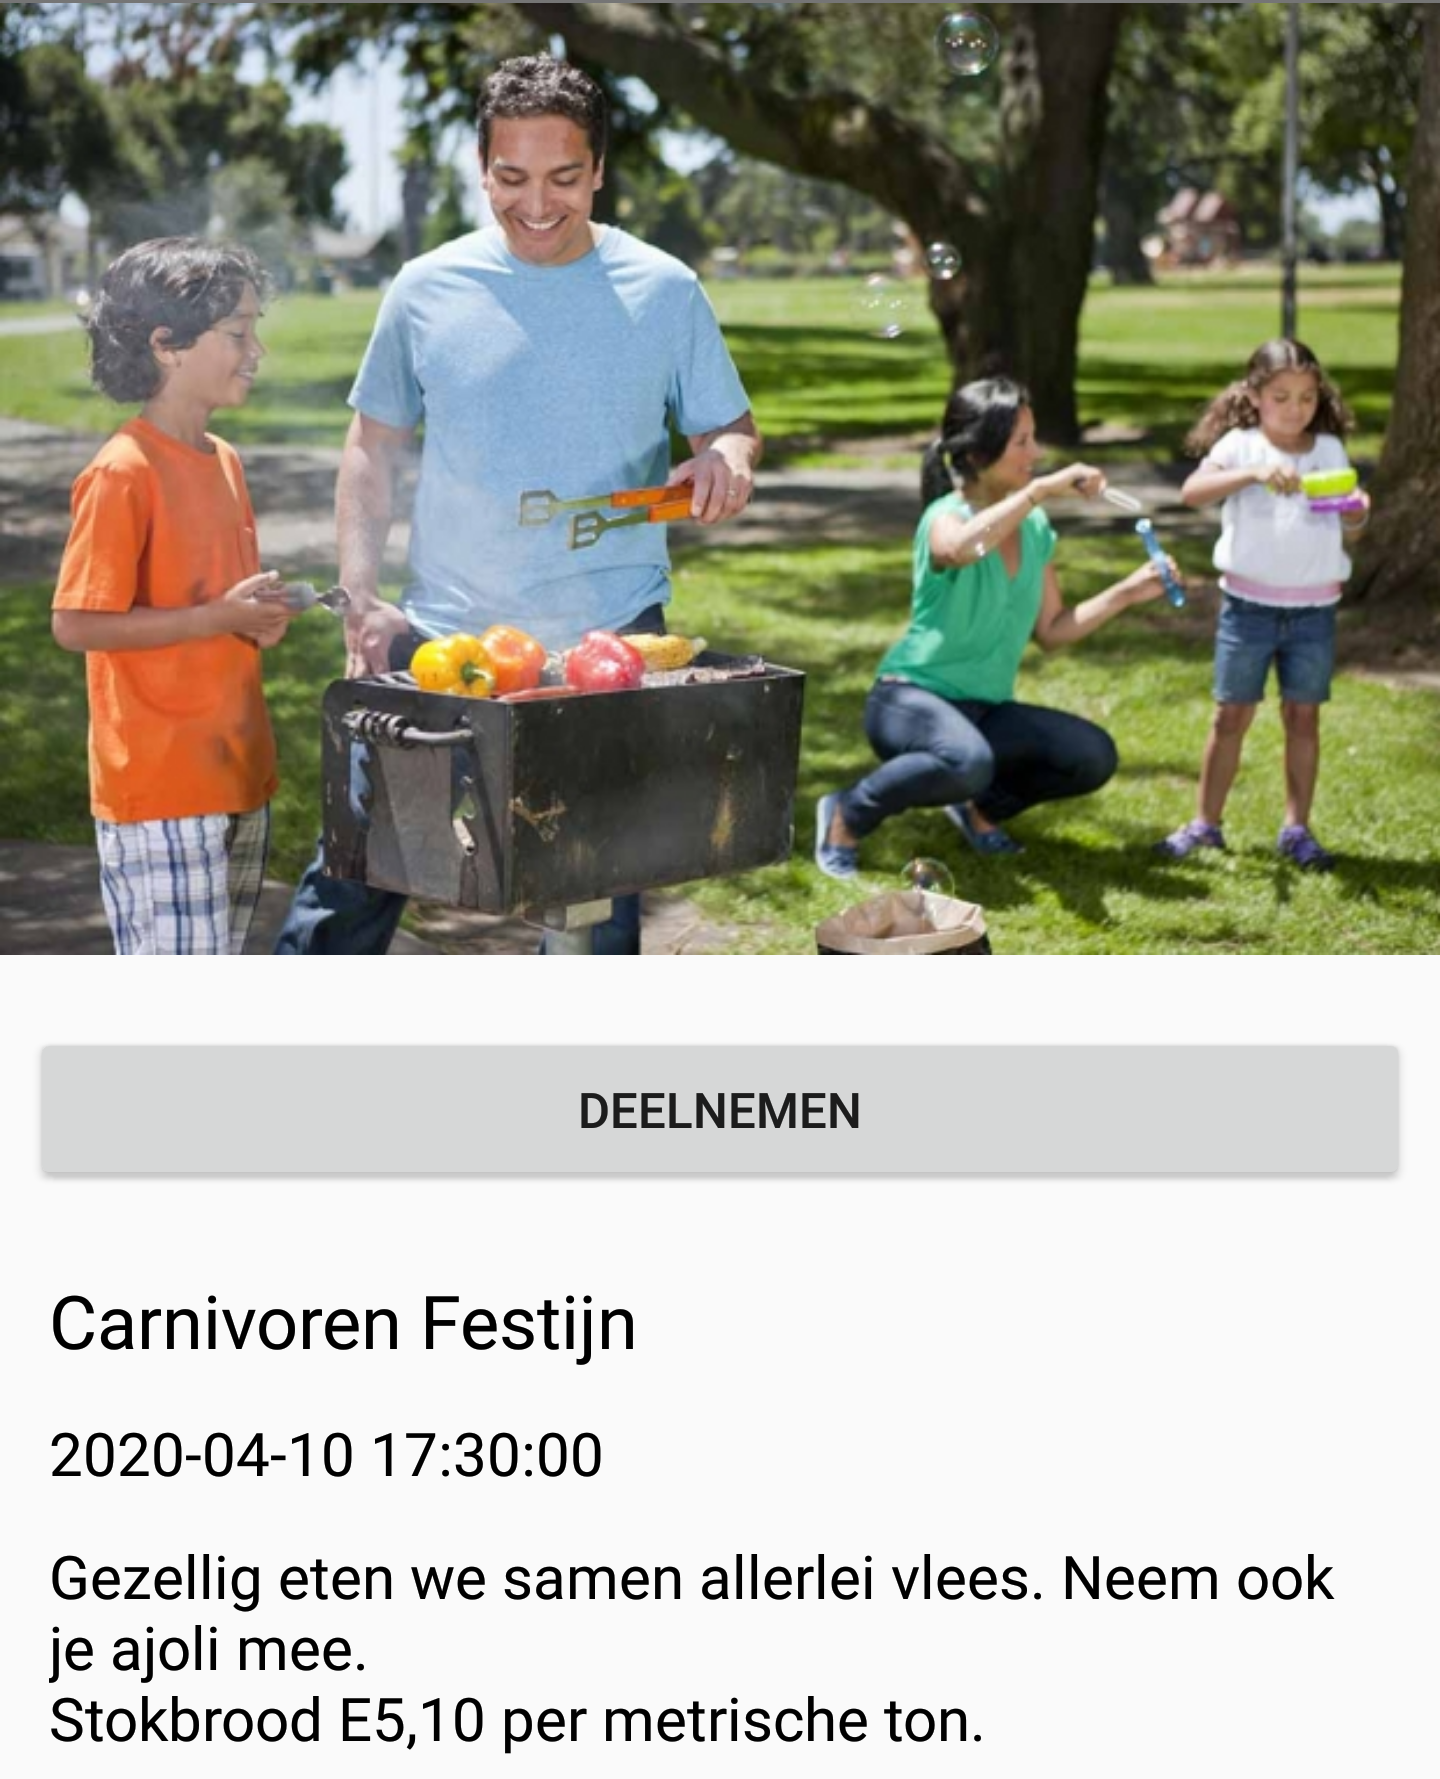
\includegraphics[width=\linewidth]{images/detailview.png}
	\end{minipage}
	
	\subsection{Het icoon}
	Voor de app is zowel een schaalbaar icoon gemaakt als een set 'ouderwetse' iconen. Met het gekke vector
	formaat dat Android gebruikt is dit niet even gemakkelijk. 


	\begin{minipage}{0.50\textwidth}
		\begin{center}
			
\includegraphics[width=2cm]{images/ic_launcher_round.png}
		\end{center}
	\end{minipage}
	\hfill
	\begin{minipage}{0.50\textwidth}
		\begin{center}
			
\includegraphics[width=2cm]{images/ic_launcher.png}
		\end{center}
	\end{minipage}	
	

	
	\section{De backend}
	%% Er is een beschrijving van de backend. Welke calls kan de API afhandelen, hoe werkt de API, waar 
	%% wordt de data opgeslagen. Waarom is er gekozen voor deze manier van dataopslag?Dit onderdeel mag 
	%% ook de beschrijving van de Firebase toepassing zijn.Er moet een vorm van persistente dataopslag 
	%% gemaakt worden.Tevens beschrijf je in hoeverre de app off-line kan werken.Het beschrijvenvande 
	%% backend, het lezen uitde backenden het schrijven naar de backend zijn onderdelen van de opdracht
	
	\section{Eigen inbreng}
	%% Eigen toevoeging aan de app. Een onderdeel wat niet in de les is besproken, maar welke de student 
	%% zelf heeft uitgezocht. Wat dat onderdeel doet, inclusief bronvermelding, wordt kort besproken. 
	%% Dit kunnen bijvoorbeeld zijn;hamburger menumaken, gebruik van fragments, animaties, externe 
	%% libraries gebruiken e.d.Als je wireframes hebt gemaakt voor het ontwerpen van je app mag je deze 
	%% ook aanleveren.
	
	\section{Git}
	%% De link naar de GIT repository met een beschrijving van de gebruikte branches. 
	
	\section{Bronnenlijst}
	%% Bronnenlijst van alle gebruikte websites, literatuur en andere bronnen
	
	\newpage
	\section{Individueel}
	
	\subsection{Roel}

	\subsubsection{Aandeel in de app}
	% De student beschrijft welke delen van de app door hem/haar gemaakt zijn.Dit is terug te vinden in de branches van de GIT-omgeving
	\subsubsection{Reflectie op de samenwerking}
	% Reflectie over de samenwerking en het leerproces van de student
	\subsubsection{Aanbeveling}
	% Aanbeveling over de module op inhoudelijk gebied: de student adviseert welke onderwerpen van applicatieontwikkeling moeten blijven 
	% in het aangeboden onderwijs en welke onderwerpen wenselijk zijn die niet zijn aangeboden, inclusief relevante verwijzingen naar
	% ondersteunende artikelen
	
	\subsection{Mies}

	\subsubsection{Aandeel in de app}
	% De student beschrijft welke delen van de app door hem/haar gemaakt zijn.Dit is terug te vinden in de branches van de GIT-omgeving
	\subsubsection{Reflectie op de samenwerking}
	% Reflectie over de samenwerking en het leerproces van de student
	\subsubsection{Aanbeveling}
	% Aanbeveling over de module op inhoudelijk gebied: de student adviseert welke onderwerpen van applicatieontwikkeling moeten blijven 
	% in het aangeboden onderwijs en welke onderwerpen wenselijk zijn die niet zijn aangeboden, inclusief relevante verwijzingen naar
	% ondersteunende artikelen	


\end{document}